\section{Accepted Configurations}
\label{sec:AcceptedConfigurations}
For every Monte Carlo cycle in the Ising model, a number, that corresponds to the number of spins in the lattice, of spin flips are proposed. 
These proposed spin flips give rise to a change in energy $\Delta E$, and the proposal is only accepted if the probability $exp(-\Delta E /T)$ is greater than some random number between 0 and 1, as explained in \secref{sec:IsingModelNgreater}. 
This gives rise to the fact that if the temperature $T$ is increased, more flips will be accepted, since then the fraction $\Delta E / T$ will decrease, which can be seen in the figures below.  
\begin{figure}[H]
\centering
\begin{minipage}{.5\textwidth}
  \centering
  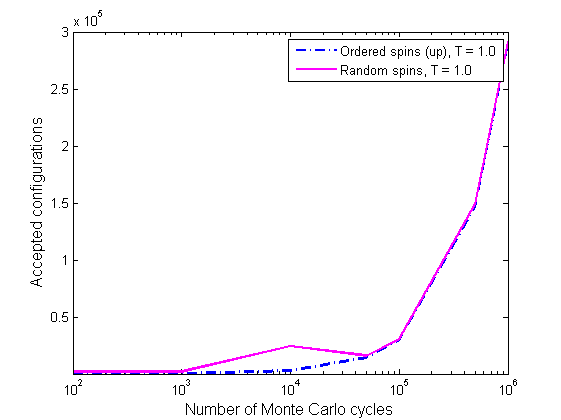
\includegraphics[width=1\linewidth]{Figures/AcceptMC_ordered_random_spins_10.png}
\end{minipage}%
\begin{minipage}{.5\textwidth}
  \centering
  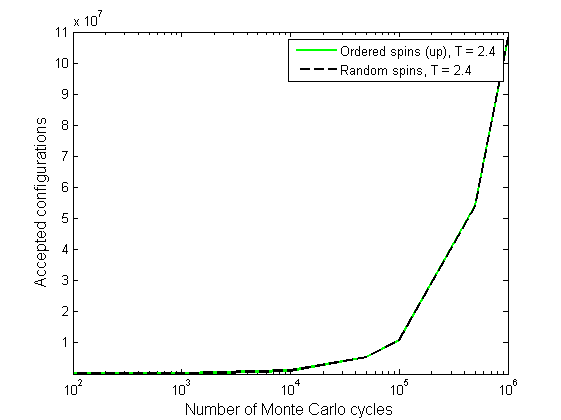
\includegraphics[width=1\linewidth]{Figures/AcceptMC_ordered_random_spins_24.png}
\end{minipage}
\caption{
Evolution of accepted spin configuration changes with ordered and random initial spin configurations for the $20\times 20$ spin case for both $T=1.0$ and $T=2.4$.
For a low number of Monte Carlo cycles the number of accepted configuration for the $T=1.0$ case is greater with the random initial spin configuration than with the ordered initial spin configuration which is in agreement with \figref{fig:ResultsMCcyclesExpectationValue1} from which it is seen that the steady state for $T=1.0$ is reached way quicker if the initial configuration of the spins is ordered. 
However, a while after having reached the steady state, the number of accepted configurations is similar for the ordered and random initial spin configuration. 
For $T=2.4$ the number of accepted configurations is similar for ordered and random initial spin configurations independently on the number of Monte Carlo cycles.  
}
\label{fig:AcceptedConfigurations1}
\end{figure}

\begin{figure}[H]
\centering
\begin{minipage}{.5\textwidth}
  \centering
  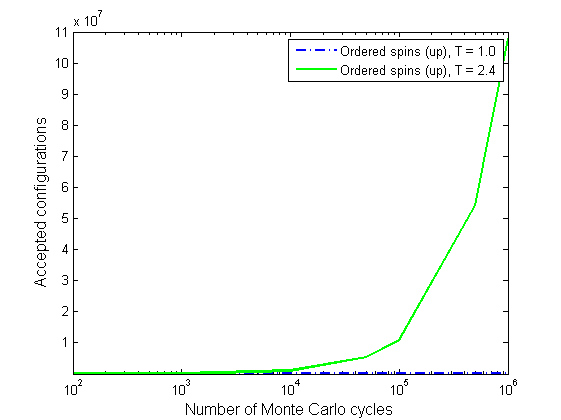
\includegraphics[width=1\linewidth]{Figures/AcceptMC_ordered_spins_10_24.png}
\end{minipage}%
\begin{minipage}{.5\textwidth}
  \centering
  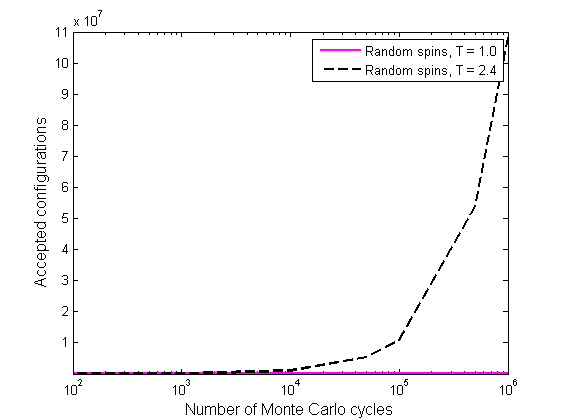
\includegraphics[width=1\linewidth]{Figures/AcceptMC_random_spins_10_24.png}
\end{minipage}
\caption{
Evolution of accepted spin configuration changes for $T=1.0$ and $T=2.4$ plotted for both ordered initial spin configurations and random initial spin configurations. 
From the plots it is evident that fewer proposed spin configuration changes are accepted for low temperature than for higher temperature. 
This is due to the fact that the probability of accepting a spin flip that causes an increase in energy is greater for higher temperature as described in \secref{sec:ResultsMCcyclesExpectationValue}, and hence more spin flips will be made for higher temperature.  
}
\label{fig:AcceptedConfigurations2}
\end{figure}